\chapter{Задание}
\section{Цель работы}
\textbf{Цель работы:} построение гистограммы и эмпирической функции распределения.
\section{Содержание работы}
\begin{enumerate}
	\item Для выборки объёма $n$ из генеральной совокупности $X$ реализовать в виде программы на ЭВМ
	\begin{enumerate}
		\item вычисление максимального значения $M_{\max}$ и минимального значения $M_{\min}$;
		\item размаха $R$ выборки;
		\item вычисление оценок $\hat\mu$ и $S^2$ математического ожидания $MX$ и дисперсии $DX$;
		\item группировку значений выборки в $m = [\log_2 n] + 2$ интервала;
		\item построение на одной координатной плоскости гистограммы и графика функции плотности распределения вероятностей нормальной случайной величины с математическим ожиданием $\hat{\mu}$ и дисперсией $S^2$;
		\item построение на другой координатной плоскости графика эмпирической функции распределения и функции распределения нормальной случайной величины с математическим ожиданием $\hat{\mu}$ и дисперсией $S^2$.
	\end{enumerate}
	\item Провести вычисления и построить графики для выборки из индивидуального варианта.
\end{enumerate}


\chapter{Теоретическая часть}
\section{Формулы для вычисления величин $M_{max}$ , $M_{min}$, R, $\hat\mu$, $S^2$}
Минимальное значение выборки рассчитывается по формуле (\ref{eq:min}); максимальное -- (\ref{eq:max}). Размах выборки рассчитывается по формуле (\ref{eq:diff}); выборочное среднее -- (\ref{eq:mx}), исправленная выборочная дисперсия -- (\ref{eq:dx}).
\begin{equation}
	\label{eq:min}
	M_{\min} = X_{(1)}
\end{equation}
\begin{equation}
	\label{eq:max}
	M_{\min} = X_{(n)}
\end{equation}
\begin{equation}
	\label{eq:diff}
	R = M_{\max} - M_{\min}.
\end{equation}
\begin{equation}
	\label{eq:mx}
	\hat\mu(\vec X_n) = \frac 1n \sum_{i=1}^n X_i
\end{equation}
\begin{equation}
	\label{eq:dx}
	S^2(\vec X_n) = \frac 1{n - 1} \sum_{i=1}^n (X_i-\overline X_n)^2
\end{equation}

\section{Эмпирическая плотность и гистограмма}
Пусть $\vec x$ -- выборка из генеральной совокупности $X$. 

При большом объеме n (n > 50) этой выборки  значения $x_i$ группируют в интервальный статистический ряд. Для этого отрезок $J = [x_{(1)}, x_{(n)}]$ делят на $m$ равновеликих промежутков по формуле (\ref{eq:ji}):

\begin{equation}
	\label{eq:ji}
	J_i = [x_{(1)} + (i - 1) \cdot \Delta,\ x_{(1)} + i \cdot \Delta), i = \overline{1; m - 1}
\end{equation}
Последний промежуток определяется по формуле (\ref{eq:jm}):
\begin{equation}
	\label{eq:jm}
	J_{m} = [x_{(1)} + (m - 1) \cdot \Delta, x_{(n)}]
\end{equation}

Ширина каждого из таких промежутков определяется по формуле (\ref{eq:delta}).
\begin{equation}
	\label{eq:delta}
	\Delta = \frac{|J|}{m} = \frac{x_{(n)} - x_{(1)}}{m}
\end{equation}

Интервальным статистическим рядом называют таблицу \ref{table:row1}:

\begin{table}[ht!]
	\captionsetup{singlelinecheck = false, justification=centering}
	\caption{Интервальный статистический ряд}
	\centering
	\label{table:row1}
	\begin{tabular}{|c|c|c|c|c|}
		\hline
		$J_1$ & ... & $J_i$ & ... & $J_m$ \\
		\hline
		$n_1$ & ... & $n_i$ & ... & $n_m$ \\
		\hline
	\end{tabular}
\end{table}

где $n_i$ -- количество элементов выборки $\vec x$, которые $\in J_i$.

\textbf{Гистограмма} -- это график эмпирической плотности. 

\textbf{Эмпирической плотностью}, отвечающей выборке $\vec x$, называют функцию:
\begin{equation}
	\hat f(x) =
	\begin{cases}
		\frac{n_i}{n \Delta}, x \in J_i, i = \overline{1; m} \\
		0\ \ , x \not\in J \\
	\end{cases}
\end{equation}

где $J_i$ -- полуинтервал статистического ряда, 
$n_i$ -- количество элементов выборки, входящих в полуинтервал, 
$n$ -- количество элементов выборки.


\section{Эмпирическая функция распределения}

Пусть $\vec x = (x_1, ..., x_n)$ -- выборка из генеральной совокупности $X$. 

Обозначим $n(t, \vec x)$ -- число элементов вектора $\vec x$, которые имеют значения меньше $t$.

\textbf{Эмпирической функцией распределения} называют функцию \newline
$F_n: \mathbb{R} \to \mathbb{R}$, определенную как: 

\begin{equation}
	F_n(t) = \frac{n(t, \vec x)}{n}
\end{equation}


\chapter{Практическая часть}
\section{Код программы}
\begin{lstlisting}[label=lst:code, caption=Программа для MatLAB, basicstyle=\footnotesize]
file = fopen('selection.txt', 'r');
X = fscanf(file, '%f,');
fclose(file);
%% Calculation
M_max = max(X);
M_min = min(X);
R = M_max - M_min;
n = length(X);
mu = sum(X) / n;
Ssquare = sum((X - mu).^2) / (n - 1);
m = floor(log2(n)) + 2;
step = R / m;
sorted_X = sort(X);
intervals = cell(1, m);
i = 1;
for cur = (M_min + step):step:M_max
    last = cur - step;
    intervals(i) = {X((last < X) & (X < cur))};
    i = i + 1;
end
intervals{m} = [intervals{m}; X(X == M_max)];
density = 1:m;
for i = 1:m
    density(i) = length(intervals{i}) / n / step;
end
%% probability density function
histogram(X, m, 'BinEdges', M_min:step:M_max, 'Normalization', 'pdf');
hold on;
x = (M_min - step):0.1:(M_max+step);
f = pdf('Normal', x, mu, Ssquare);
plot(x,f,'LineWidth',1.5, 'color', 'red')
hold off;
%% probability function
x = (M_min - step):0.1:(M_max+step);
[F_empirical, x_empirical] = ecdf(X);
F = normcdf((x - mu) / sqrt(Ssquare));
hold on;
plot(x_empirical, F_empirical,'LineWidth', 1.5);
plot(x, F,'LineWidth', 1.5, 'color', 'red');
hold off;
\end{lstlisting}

\newpage
\section{Результаты расчетов для выборки из индивидуального варианта.}
Согласно варианту 3, результаты расчетов для выборки приведены на формулах (\ref{eq:res_min}), (\ref{eq:res_max}), (\ref{eq:res_r}), (\ref{eq:res_mx}), (\ref{eq:res_dx}), (\ref{eq:res_m}).
\begin{equation}
	\label{eq:res_min}
	M_{\min} = -2.77
\end{equation}
\begin{equation}
	\label{eq:res_max}
	M_{\max} = 2.92
\end{equation}
\begin{equation}
	\label{eq:res_r}
	R = 5.69
\end{equation}
\begin{equation}
	\label{eq:res_mx}
	\hat\mu(\vec x_n) = 0.2323
\end{equation}
\begin{equation}
	\label{eq:res_dx}
	S^2(\vec x_n) = 1.0406
\end{equation}
\begin{equation}
	\label{eq:res_m}
	m = 8
\end{equation}

На рисунке \ref{image:graph1} представлены гистограмма и график функции плотности распределения вероятностей нормальной случайной величины с выборочными мат. ожиданием и дисперсией.
\begin{figure}[h]
	\centering{
		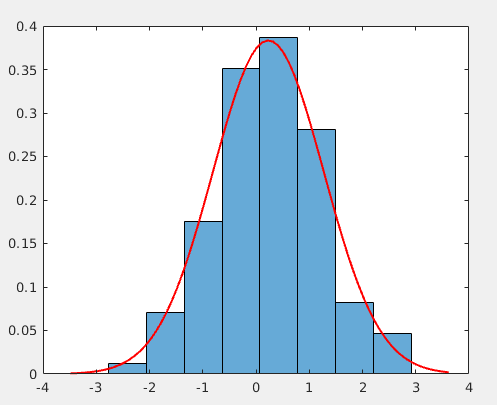
\includegraphics[scale=0.5]{./img/graph1}
		\caption{Гистограмма и график функции плотности распределения вероятностей нормальной случайной величины с выборочными мат. ожиданием и дисперсией.}
		\label{image:graph1}
	}
\end{figure}

\clearpage
На рисунке \ref{image:graph2} представлены график эмпирической функции распределения и функции распределения нормальной случайной величины с выборочными мат. ожиданием и дисперсией.
\begin{figure}[h]
	\centering{
		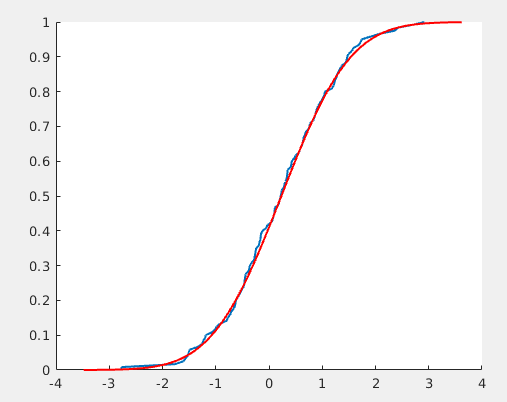
\includegraphics[scale=0.5]{./img/graph2}
		\caption{График эмпирической функции распределения и функции распределения нормальной случайной величины с выборочными мат. ожиданием и дисперсией.}
		\label{image:graph2}
	}
\end{figure}


